\documentclass[a4paper]{article}
\usepackage{float}

\usepackage{amsmath}
\usepackage{amssymb}
\usepackage{graphicx}
\usepackage{inputenc}
\usepackage{hyperref}
\usepackage{listings}
\usepackage{polski}

\title{Raport}
\author{Łukasz Fabia}
\date{20.05.2024}

\begin{document}

\maketitle
\tableofcontents

\section{Wstęp}

\quad Celem badań jest analiza danych dotyczących ofert pracy w IT. W swojej pracy postaram się
odpowiedzieć na pytanie, jakie są najbardziej poszukiwane umiejętności w branży IT oraz ile można zarobić
znając dane języki, frameworki czy narzędzia. W tym celu postram się wykorzystać sci-kit learn do stworzenia
modelu regresji liniowej, który pozwoli mi przewidzieć zarobki na podstawie umiejętności (technologii).


\section{Dane}

\quad Dane pozyskam z serwisu \href{https://justjoin.it/}{justjoin.it}, który zbiera oferty pracy z wielu różnych serwisów, zatem
ofert pracy będzie całkiem sporo. Na stronie mamy katergorie, które mogą być przydatne do analizy, takie jak:
JS, PHP, Ruby, Python, Java, Net, Mobile, C, DevOps, Security, Data, Go, Game, Scala. W mojej analizie skupię się na nich.
\quad Dodatkowo analizuję zarobki tylko na b2b oraz na umowie o prace (uop), ponieważ są to najbardziej popularne formy zatrudnienia w IT a inne formy takie jak umowa
o zlecenie czy umowa o staż pratykcznie nie występują. Do analizy będę również brał pod uwagę lokalizację.

\textbf{\newline Technologia} - język programowania, framework, narzędzie, które jest wymagane w ofercie pracy.

\subsection{Model danej}
\quad Dane będą zawierały informacje o ofertach pracy, takie jak:
\begin{itemize}
    \item tytuł oferty
    \item widełki dla B2B
    \item widełki dla UOP
    \item technologie dotyczące umowy
    \item lokalizacja
    \item doświadczenie {junior, mid, senior}
    \item typ pracy {stacjonarnie, hybrydowo, zdalnie}
\end{itemize}

\subsection{Obsługa technologii, lokalizacji}

\quad Najpierw zdefiniuje sobie słownik klucz, wartość, gdzie klucz to ustandaryzowana technologia, a wartość do synonimy tej technologii.

\textit{np. \ "JavaScript": [
"javascript",
"js",
"node.js",
"nodejs",
"express.js",
"expressjs",
],}

\quad Dzięki temu będę mógł przekonwertować technologie z oferty pracy na wektor binarny, gdzie 1 oznacza, że technologia jest wymagana, a 0, że nie jest wymagana. Kolejnym
krokiem będzie obsługa lokalizacji. W tym przypadku jeśli oferta dot. kilku miast to znaczy, że pojawi się w zbiorze
klika ofert z tymi samymi danymi, ale dla różnych miast.


\subsection{Pozykiwanie danych}

\quad Dane będą pozyskiwane z ww. serwisu, za pomocą narzędzi do web scrappingu w moim przypadku będzie
to \texttt{Selenium}, ponieważ strona ma dynamicznie ładowany content.


Kroki:
\begin{itemize}
    \item napisanie skryptu pobierającego linki do ofert pracy z danej kategorii, ponieważ nie chcemy śmiecowych ofert typu Product manager
    \item napisanie skryptu przetwarzającego linki do ofert pracy, aby pobrać dane z oferty
    \item przekierowanie wyniku do pliku json.
    \item normalizacja oraz oczyszczanie danych, kodowanie technologii, do wektora przy pomocy MultiLabelBinarizer z \texttt{sklearn}
    \item kodowanie duplkacja ofert z różnymi lokalizacjami oraz kodowanie typu pracy i doświadczenia (\texttt{label encoding})
    \item usunięcie ofert z wynagrodzniem godzinowym bo zalezą one od ilości przepracowanych godzin
\end{itemize}

\textit{Ofert ze stawką godzinową było kilka więc nie wypływają one na wyniki.}

\section{Wygląd do danych}

\textit{uwaga przykładowe dane nie zawierają wszystkich kolumn bo jest ich za dużo, wszystkie dane można znaleźć w ../data/jobs.csv}


\textbf{Przykładowe dane:}


\begin{table}[h]
    \centering
    \begin{tabular}{|c|c|c|c|c|}
        \hline
        \multicolumn{1}{|c|}{\textbf{title}} & \textbf{min\_b2b} & \textbf{max\_b2b} & \textbf{min\_uop} & \textbf{max\_uop} \\ \hline
        Senior Software Engineer             & 0.0               & 0.0               & 18000.0           & 28000.0           \\ \hline
        Senior Backend Node.js Engineer      & 0.0               & 0.0               & 18360.0           & 25125.0           \\ \hline
        Senior Fullstack Developer           & 22680.0           & 27216.0           & 16600.0           & 19920.0           \\ \hline
    \end{tabular}
\end{table}


\begin{table}[h]
    \centering
    \begin{tabular}{|c|c|c|c|}
        \hline
        \textbf{location\_code} & \textbf{operating\_mode\_code} & \textbf{experience\_code} \\ \hline
        38                      & 0                              & 2                         \\ \hline
        17                      & 2                              & 2                         \\ \hline
        51                      & 0                              & 2                         \\ \hline
    \end{tabular}
\end{table}


\begin{table}[h]
    \centering
    \begin{tabular}{|c|c|c|c|}
        \hline
        \textbf{AWS} & \textbf{JavaScript} & \textbf{React} & \textbf{Java} \\ \hline
        1            & 1                   & 1              & 0             \\ \hline
        0            & 1                   & 1              & 0             \\ \hline
        1            & 1                   & 1              & 0             \\ \hline
    \end{tabular}
\end{table}

\newpage

\section{Rozkłady i statystyki}

\quad Aktualnie w zbiorze \textit{jobs.csv} znajduje się \textbf{4574} ofert pracy, które będą poddane
analizie. Wszystkie dane są znormalizowane i gotowe do analizy. Analizę można zacząć od średniej zarobków
dla kontraktu B2B oraz UOP.


\textbf{Widełki dla Juniora: }

\begin{table}[h]
    \centering
    \begin{tabular}{|c|c|c|c|}
        \hline
        \textbf{PLN}             & \textbf{B2B} & \textbf{UOP} \\ \hline
        \textbf{średnie widełki} & 8555.40      & 13558.71     \\ \hline
        \textbf{min widełki}     & 4250.00      & 6000.00      \\ \hline
        \textbf{max widełki}     & 16443.00     & 28000.00     \\ \hline
    \end{tabular}
    \caption{Średnie zarobki w PLN dla \texttt{juniora} w Polsce}
\end{table}

\textbf{Widełki dla Mida: }

\begin{table}[h]
    \centering
    \begin{tabular}{|c|c|c|c|}
        \hline
        \textbf{PLN}             & \textbf{B2B} & \textbf{UOP} \\ \hline
        \textbf{średnie widełki} & 12378.99     & 18041.77     \\ \hline
        \textbf{min widełki}     & 5000.00      & 7000.00      \\ \hline
        \textbf{max widełki}     & 25000.00     & 30000.00     \\ \hline
    \end{tabular}
    \caption{Średnie zarobki w PLN dla \texttt{mida} w Polsce}
\end{table}

\textbf{Widełki dla Seniora: }

\begin{table}[h]
    \centering
    \begin{tabular}{|c|c|c|c|}
        \hline
        \textbf{PLN}             & \textbf{B2B} & \textbf{UOP} \\ \hline
        \textbf{średnie widełki} & 18930.61     & 25848.46     \\ \hline
        \textbf{min widełki}     & 8000.00      & 11000.00     \\ \hline
        \textbf{max widełki}     & 40000.00     & 80000.00     \\ \hline
    \end{tabular}
    \caption{Średnie zarobki w PLN dla \texttt{seniora} w Polsce}
\end{table}
\newpage
\subsection{Jak się pracuje w IT?}

\begin{figure}[H]
    \centering
    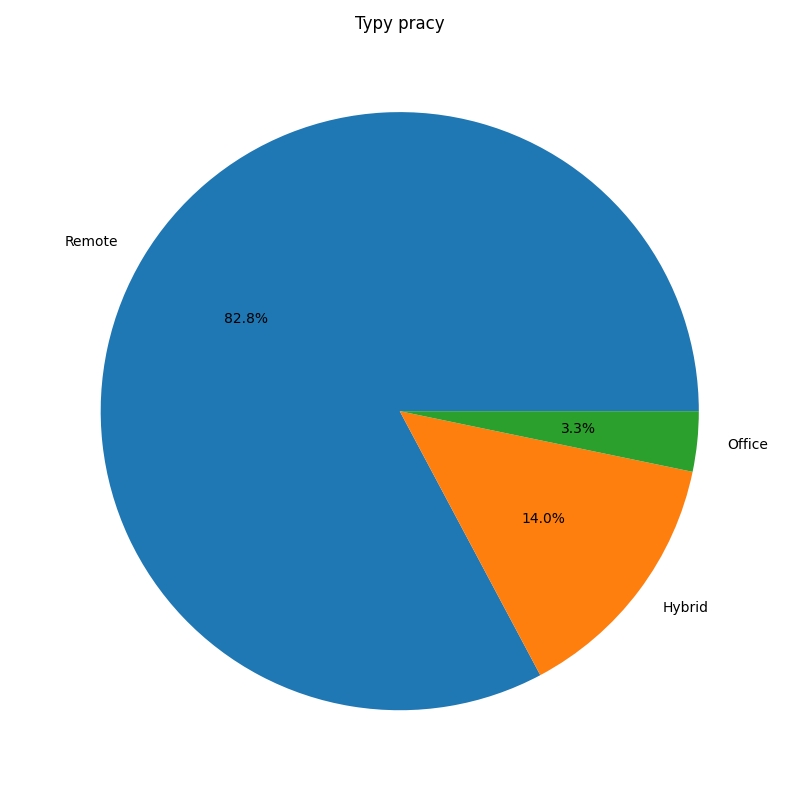
\includegraphics[width=0.8\textwidth]{../analysis/plots/rozkłady/typy_pracy.png}
    \caption{Rozkład typów pracy}
\end{figure}

\quad Jak widać najwięcej ofert pracy dotyczy pracy zdalnej.


\subsection{Kogo szukają pracodawcy?}

\begin{figure}[H]
    \centering
    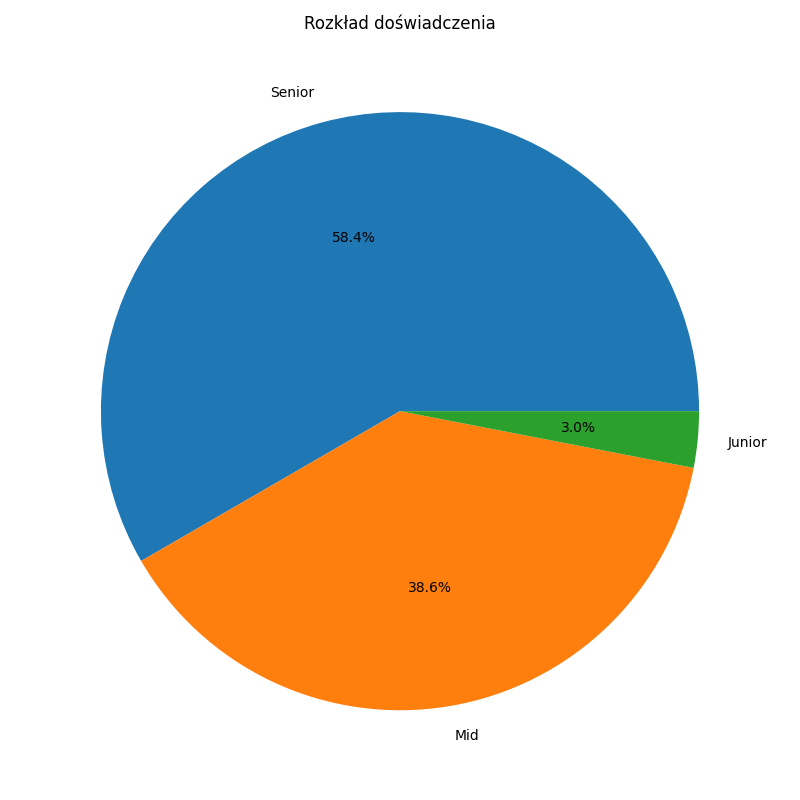
\includegraphics[width=0.8\textwidth]{../analysis/plots/rozkłady/rozkład_doświadczenia.png}
    \caption{Rozkład typów pracy}
\end{figure}

\quad Tak jak można było się spodziewać - najwięcej ofert pracy jest dla seniorów,
stąd też wynika dlaczego tak dużo kontraktów dotyczy pracy zdalnej. Chociaż
warto powiedzieć sytuacja midów jest również dobra. Gorzej jest z ofertami dla młodych programistów.
Tutaj liczba ofert wyniosła zaledwie 139, co jest bardzo małą liczbą w porównaniu do innych grup.

\textit{Czy to oznacza, że młodzi programiści mają trudniej, a słynne "eldorado" w IT jest tylko dla doświadczonych programistów?}

\quad Tutaj można powiedzieć, że juniorzy mają trudniej \textbf{wejść} do branży, ale zarobki po wejściu są naprawdę atrakcyjne,
no, ale tutaj problem może być z wejściem.


\subsection{Jak rozkładają się zarobki?}

\begin{figure}[H]
    \centering
    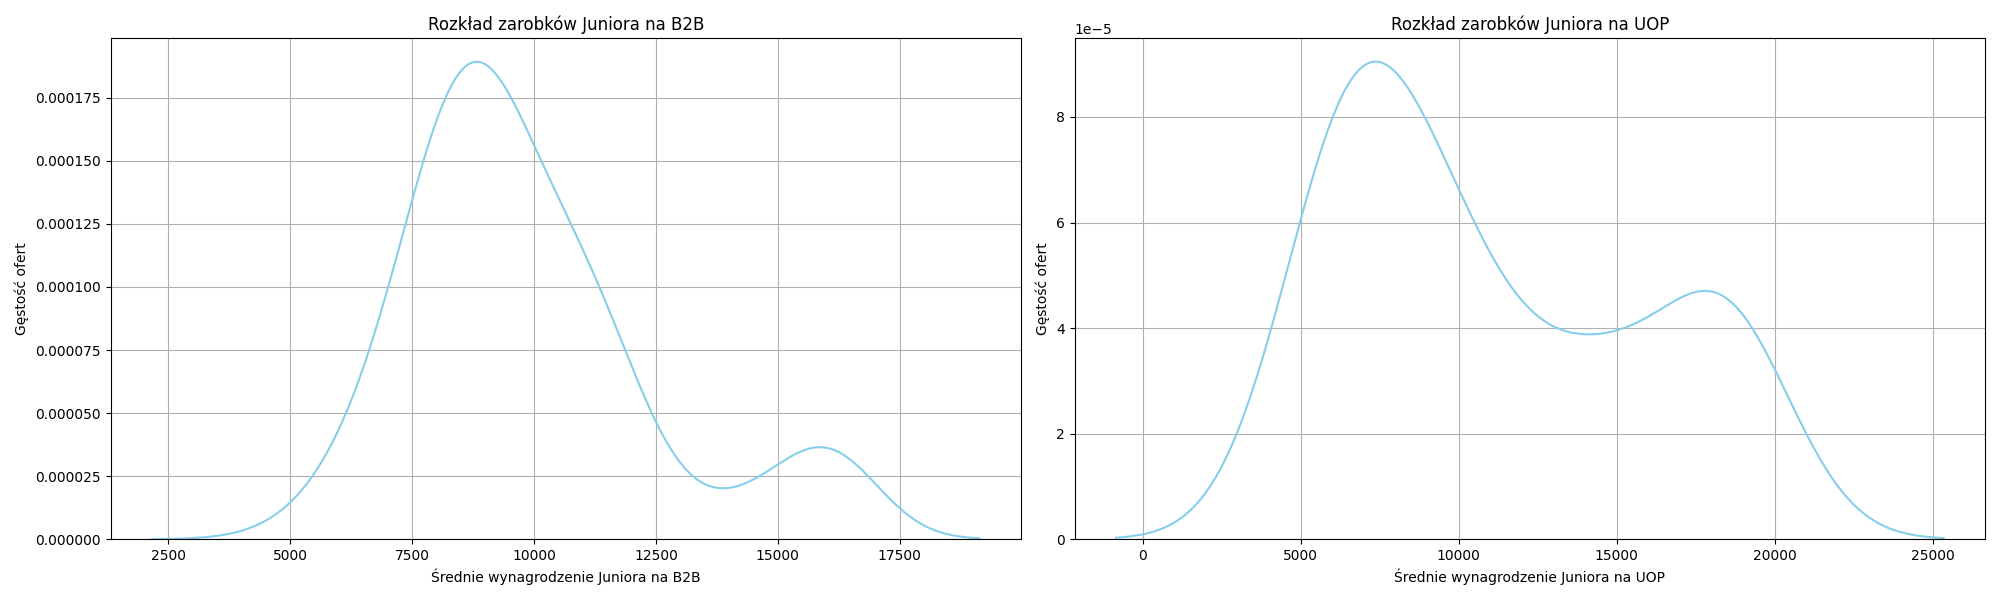
\includegraphics[width=0.8\textwidth]{../analysis/plots/rozkłady/pensje_dla_juniora.png}
    \caption{Rozkłady zarobków dla poszczególnych umów dla juniorów}
\end{figure}

\begin{figure}[H]
    \centering
    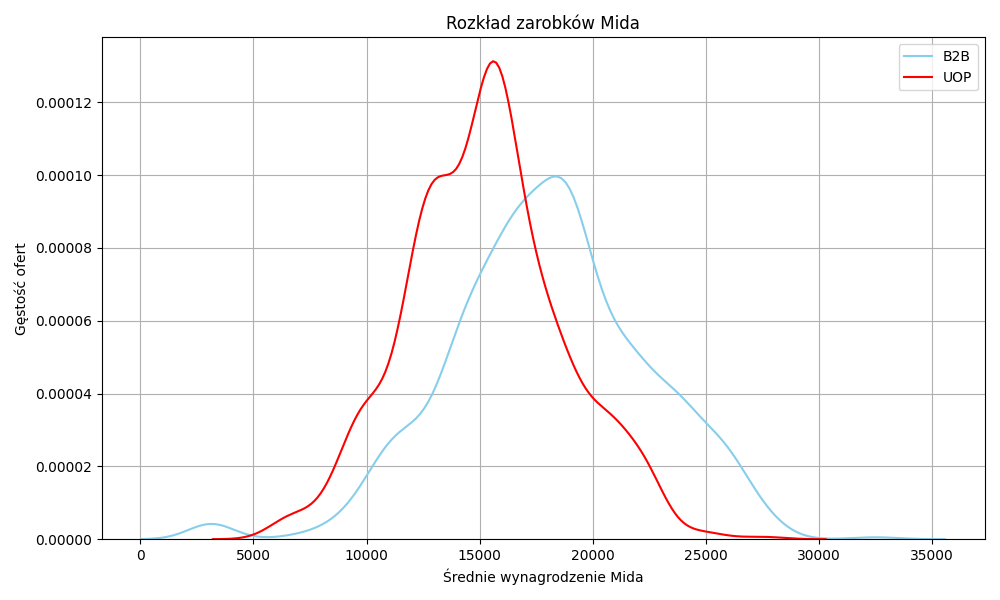
\includegraphics[width=0.8\textwidth]{../analysis/plots/rozkłady/pensje_dla_mida.png}
    \caption{Rozkłady zarobków dla poszczególnych umów dla midów}
\end{figure}

\begin{figure}[H]
    \centering
    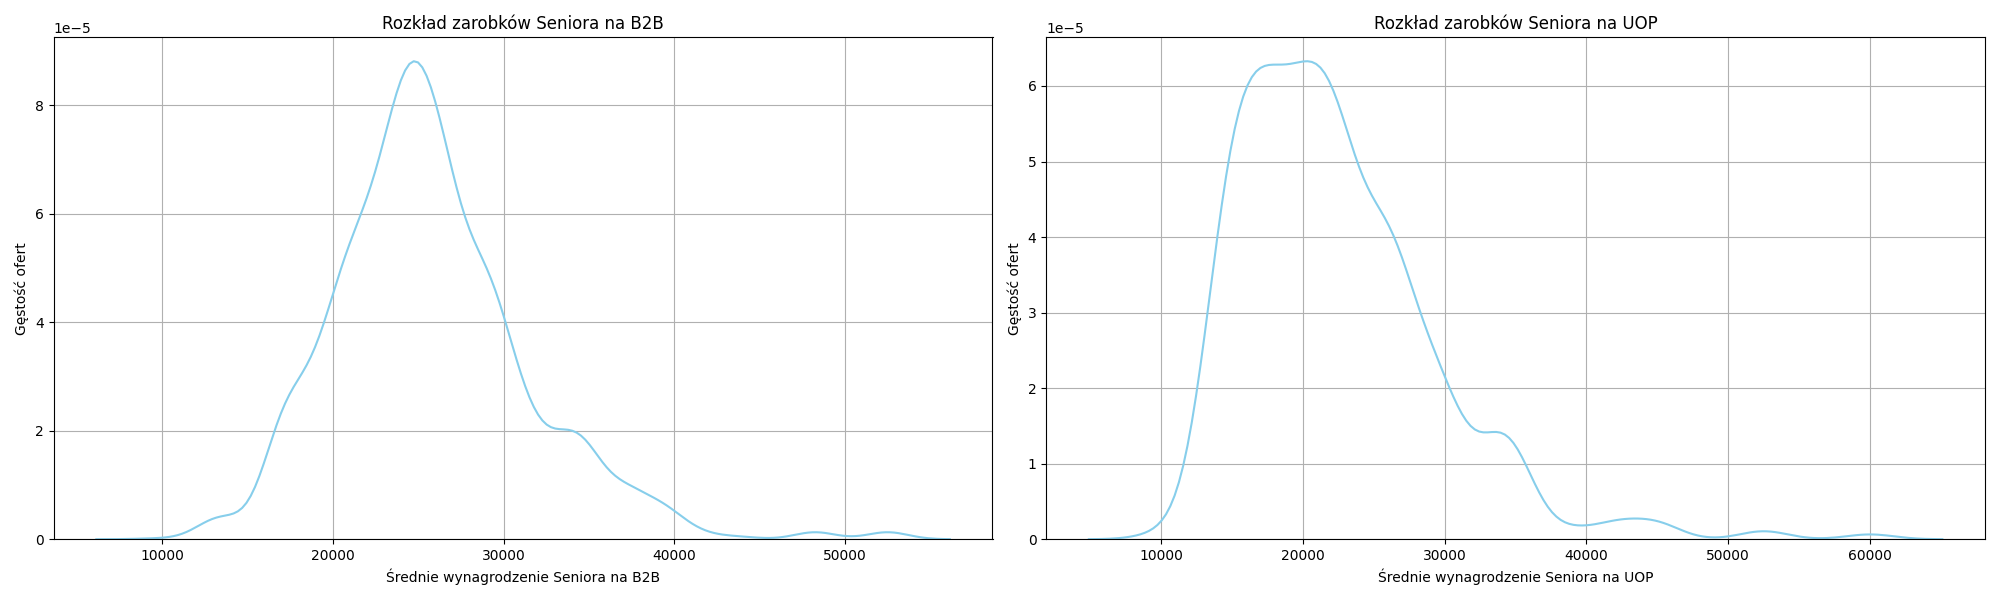
\includegraphics[width=0.8\textwidth]{../analysis/plots/rozkłady/pensje_dla_seniora.png}
    \caption{Rozkłady zarobków dla poszczególnych umów dla seniorów}
\end{figure}


\subsection{Jakie technologie są najbardziej poszukiwane?}

\begin{figure}[H]
    \centering
    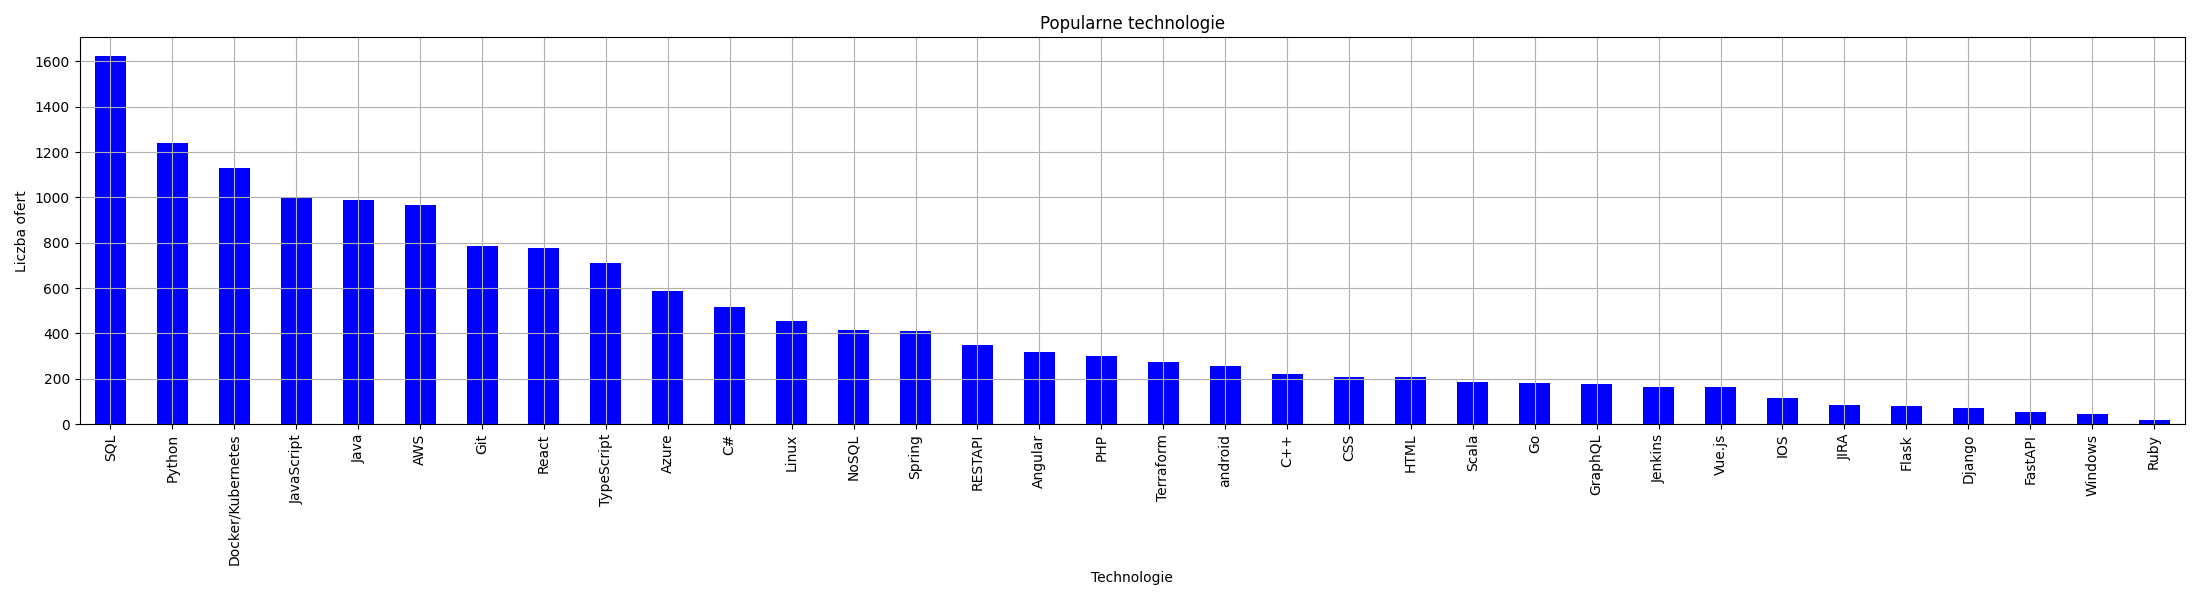
\includegraphics[width=\textwidth]{../analysis/plots/rozkłady/popularne_technologie.png}
    \caption{Popularne technologie w ofertach pracy w Polsce}
\end{figure}

\quad Tutaj moim zdaniem troche zaskoczenie ponieważ bez \texttt{SQL} ciężko znaleźć prace w IT, czyli
bazy danych to jest podstawa przy rekrutowanu się do pracy. Oczywiście nie mogło zabraknąć \texttt{Pythona} oraz \texttt{JavaScriptu} jeśli chodzi o języki skryptowe.
Co warto zazanczyć narzędzia takie jak \texttt{Docker} czy \texttt{Kubernetes} również są bardzo popularne i warto je znać. \texttt{Java} wygrywa z \texttt{C\#} a \texttt{GNU/Linux} deklasuje \texttt{Windowsa}.


\subsection{Gdzie jest największy popyt na programistów?}

\begin{figure}[H]
    \centering
    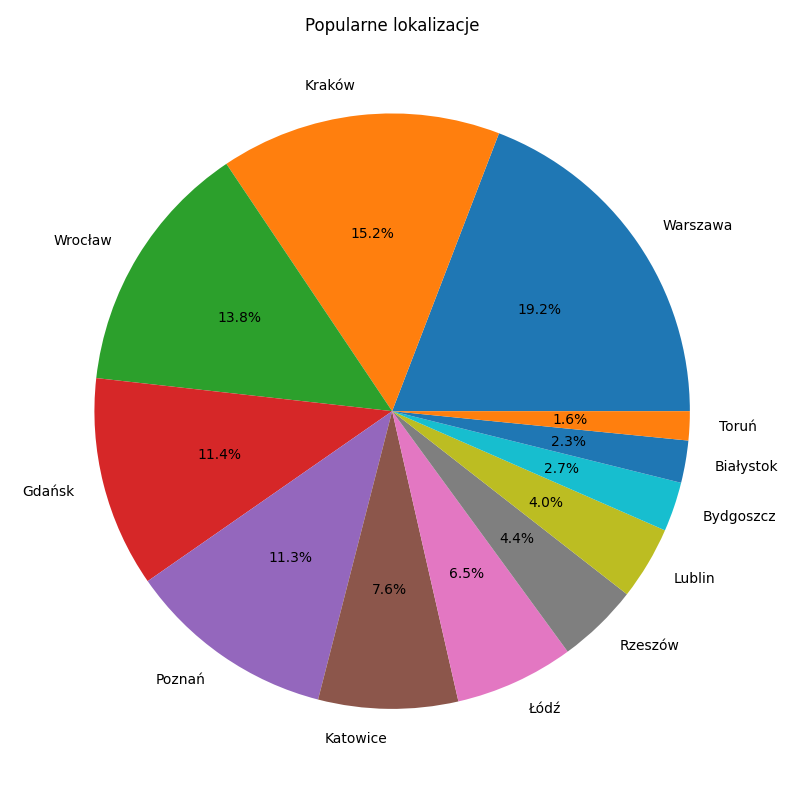
\includegraphics[width=0.8\textwidth]{../analysis/plots/rozkłady/popularne_lokalizacje.png}
    \caption{Popularne miasta w ofertach pracy w Polsce}
\end{figure}

\quad Zestawienie miast jest zgodne z oczekiwaniami, najwięcej ofert pracy jest kolejno w \textbf{Warszawie}, \textbf{Krakowie} oraz \textbf{Wrocławiu}, chociaż
\textbf{Gdańsk} również pojawiał się w dużej ilości ofert pracy.


\subsection{Gdzie poszukiwani są juniorzy?}

\begin{figure}[H]
    \centering
    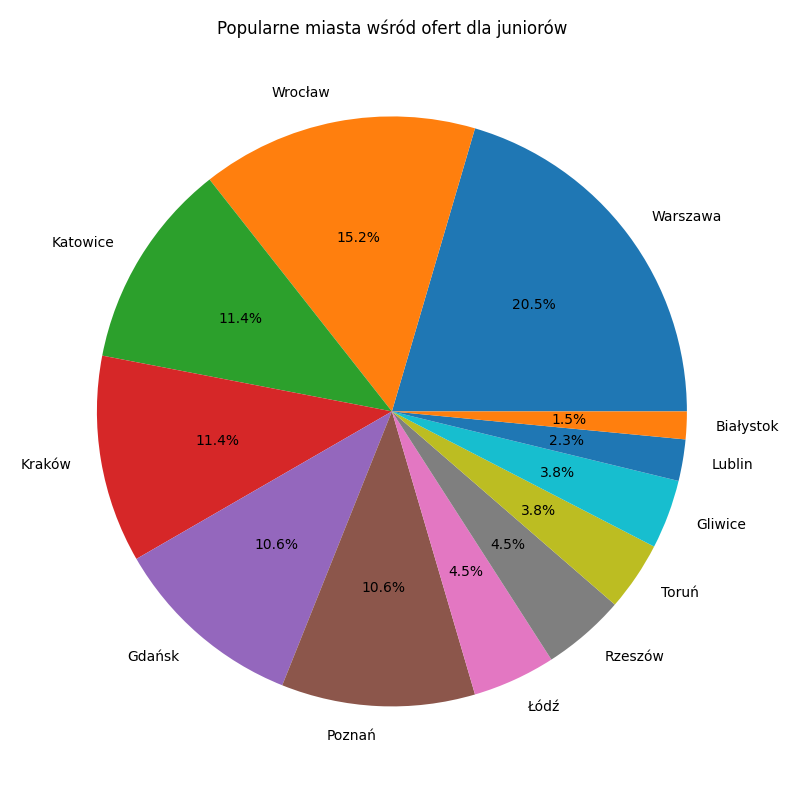
\includegraphics[width=\textwidth]{../analysis/plots/rozkłady/popularne_miasta_wśród_ofert_dla_juniorów.png}
    \caption{Popularne miasta w ofertach dla juniorów}
\end{figure}

\quad \textbf{Warszawa} jest najbardziej przyjazna dla juniorów, ale
warto zauważyć, że wykres nie różni się bardzo od poprzedniego z jednym, \textit{ale} - \textbf{Katowice} są
na 3 miejscu w zestawieniu dla juniorów, co może być zaskoczeniem.


\section{Powiązania między danymi}

\subsection{Powiązania między technologiami}

\begin{figure}[H]
    \centering
    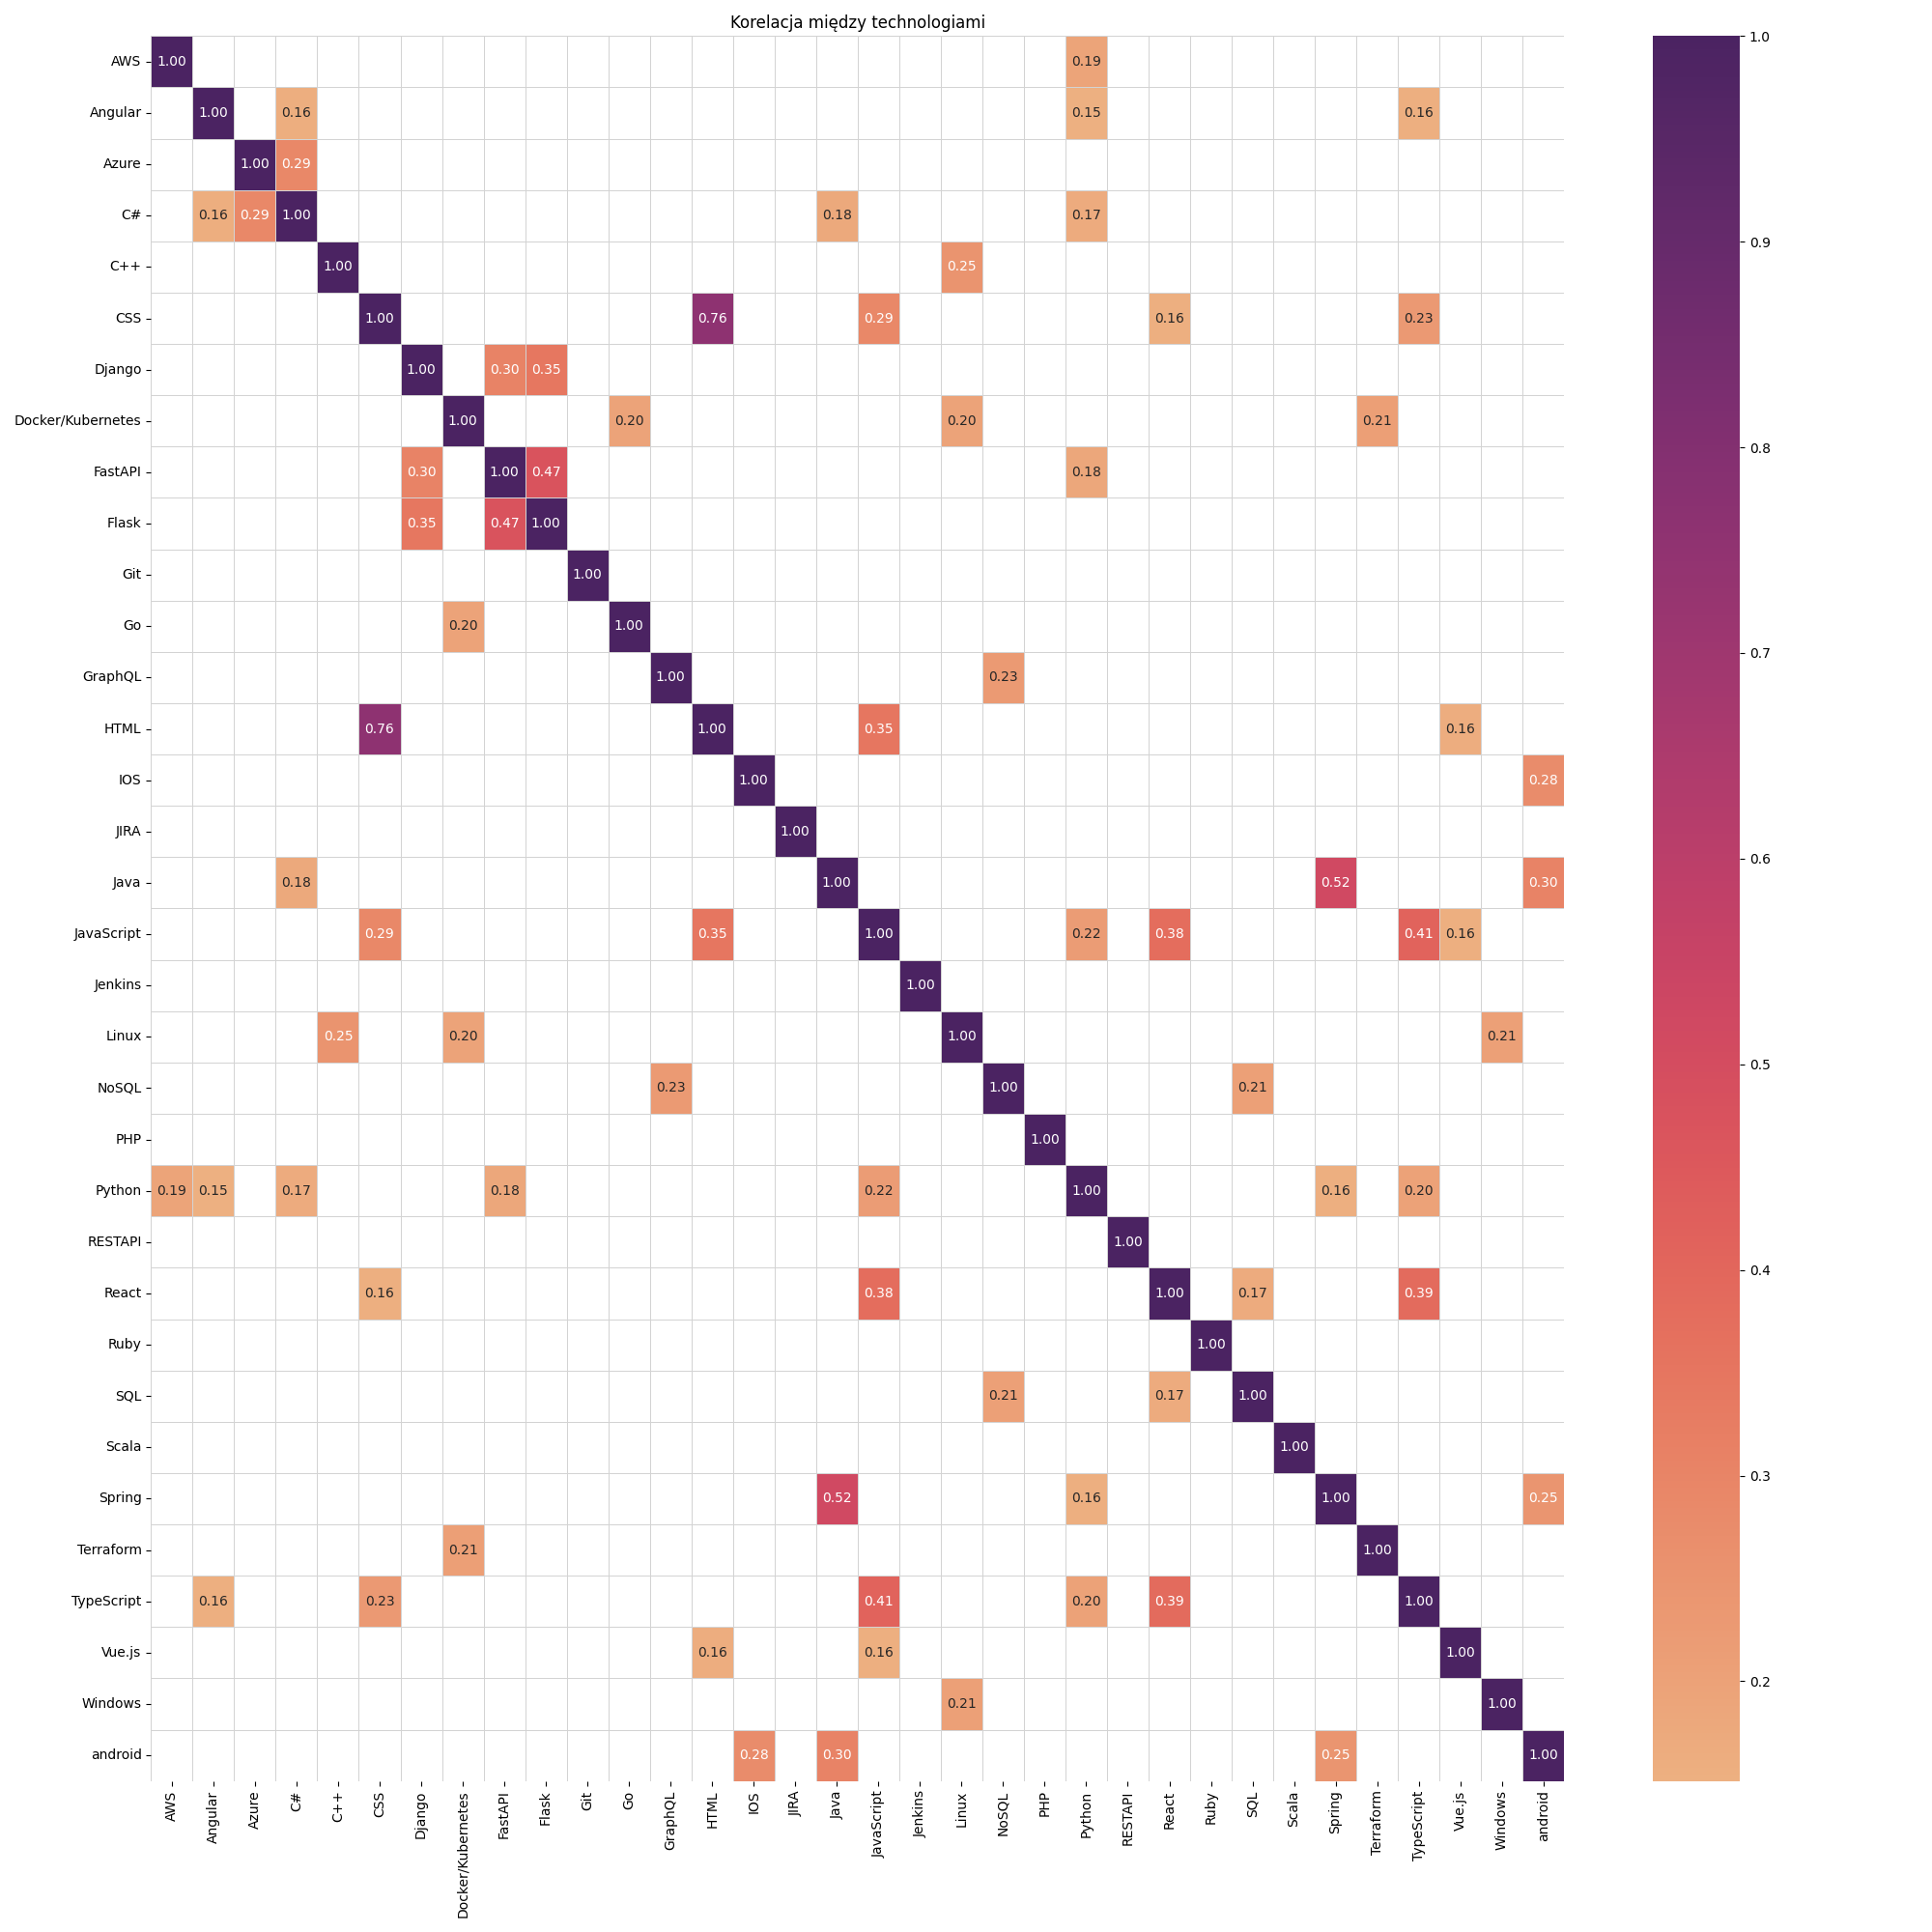
\includegraphics[width=\textwidth]{../analysis/plots/korelacje/korelacja_między_technologiami.png}
    \caption{Powiązania między technologiami, zawierająca tylko wartości korelacji większe niż 0.14}
\end{figure}

\quad \textbf{Co można zauważyć?}

\begin{enumerate}
    \item HTML i CSS idą ze prawie w parze - co jest zrozumiałe, bo to podstawy front-endu
    \item Przy Javie warto znać Springa
    \item React i JS i TS często pojawiają sie razem w ofertach pracy obok HTML i CSS
    \item Jak sie uczy Django to warto znać inne frameworki backendowe takie jak Flask czy FastAPI
    \item Jak sie idzie w Embedded to warto znać C/C++ oraz Linux
\end{enumerate}

\quad To tylko kilka przykładów wymienionych wynikający z obrazka powyżej, ale warto zauważyć, że nie ma tutaj dużo
powiązań między technologiami, co może wynikać z tego, że technologie są zbyt różne, aby były powiązane.


\subsection{Powiązania między innymi zmiennymi}

\begin{figure}[H]
    \centering
    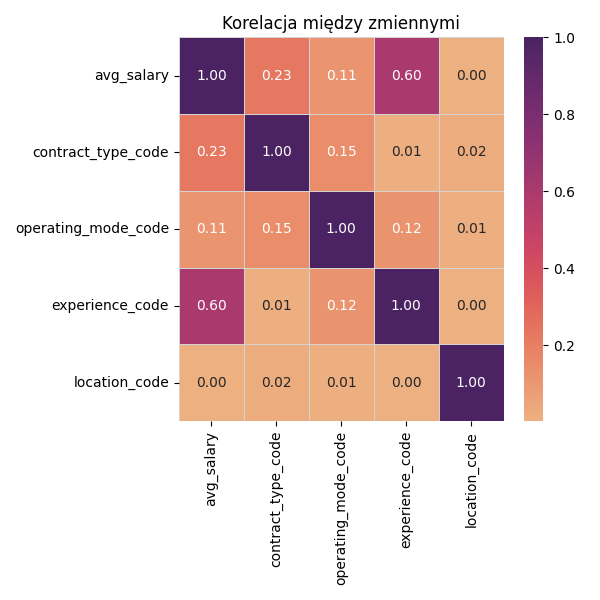
\includegraphics[width=\textwidth]{../analysis/plots/korelacje/korelacja_między_zmiennymi.png}
    \caption{Powiązania między innymi zmiennymi}
\end{figure}

\quad \textbf{Co można zauważyć?}

\begin{enumerate}
    \item W jakiś spobób powiązane są ze sobą zarobki na B2B i UOP - ma sens
    \item Wynagrodzenie na B2B i UOP jest powiązane z doświadczeniem
\end{enumerate}


\subsection{Zarobek a technologie}

\begin{figure}[H]
    \centering
    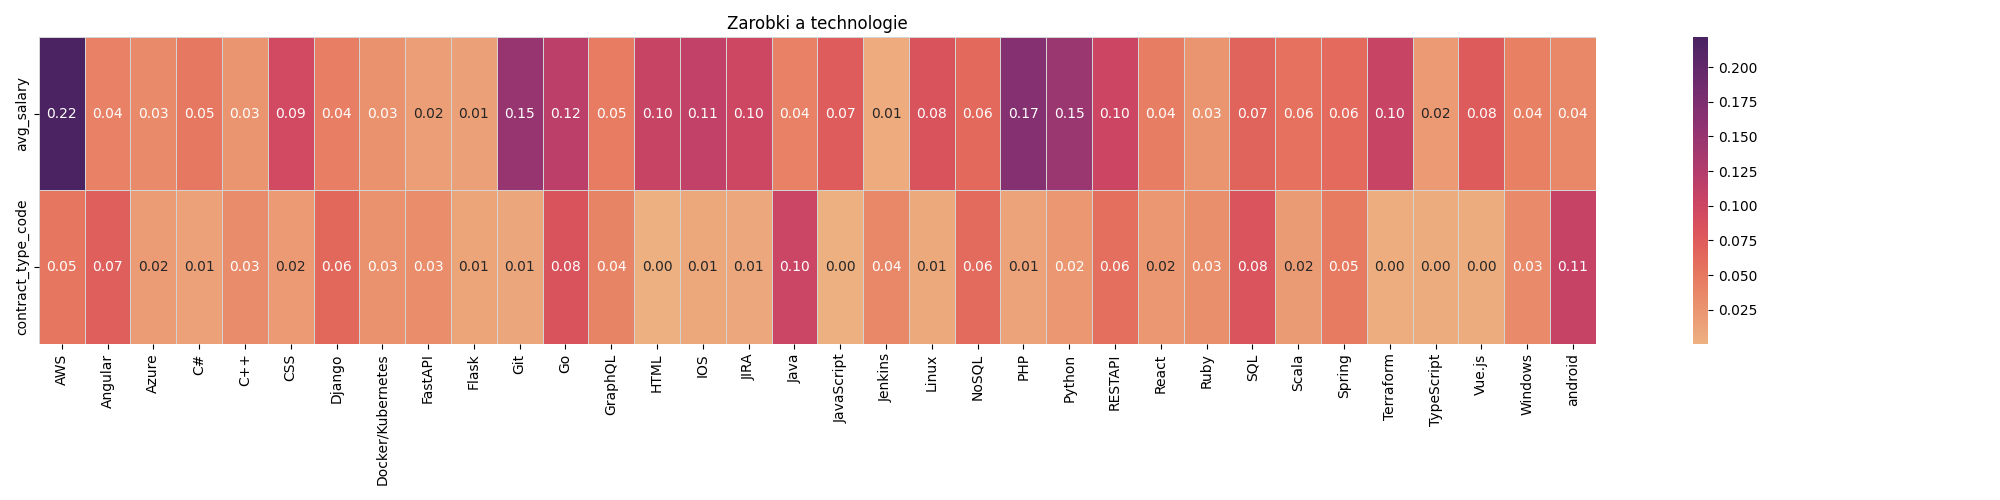
\includegraphics[width=\textwidth]{../analysis/plots/korelacje/zarobki_a_technologie.png}
    \caption{Powiązania między zarobkiem a technologiami}
\end{figure}

\quad Tutaj jest kilka ciekawych powiązań, które warto zauważyć, np. na umowie o prace znaczenie ma
znajomość: Go, AWS, Angulara, Java, SQL czy Andorida, chociaż nie są to mocne powiązania. Natomiast na B2B nie ma jakiś znaczących powiązań można wskazać
np. Resta, AWS, Docker/Kubernetes czy PHP, ale są to watości rzędu 0.09, co nie jest imponującym wynikiem.


\section{Czy da się przewidzieć zarobki, w zależności od mojego tech-stacku?}

\subsection{Ogólnie o problemie}

\quad \textbf{Oczywiście}, że tak, kiedy mamy dane to możemy nauczyć model, który na wejściu dostanie zmienne i przewidzi dla nas
zarobki. Dokładniej mówiąc model otrzyma na wejściu dane takie jak:

\texttt{Input:}

\begin{itemize}
    \item Tech-stack
\end{itemize}

\texttt{Output:}

\begin{itemize}
    \item Zarobki w PLN
\end{itemize}


\subsection{Dobór modeli}

\quad Modele które będą wykorzystane w analizie to:

\begin{enumerate}
    \item Regresja liniowa
          \begin{itemize}
              \item \texttt{LinearRegression}
              \item \texttt{Ridge}
              \item \texttt{Lasso}
              \item \texttt{ElasticNet}
          \end{itemize}
    \item \texttt{Decision tree}
    \item \texttt{Random forest}
\end{enumerate}

\textit{Wszyskie modele pochodzą z modułu \texttt{sklearn} dostępniej pod \href{https://scikit-learn.org/stable/}{tym linkiem}}

\subsection{Trochę statystyki - metryki}

\quad Do oceny modeli wykorzystam metryki takie jak:

\begin{itemize}
    \item \textbf{Root Mean Squared Error} - pierwiastek z średniego błędu kwadratowego
    \item \textbf{R-squared} - współczynnik determinacji $R^2$
    \item \textbf{Mean Absolute Error} - średni błąd bezwzględny
\end{itemize}

\subsubsection{Pierwiastek z średniego błędu kwadratowego}

\quad \textbf{Root Mean Squared Error (RMSE)} - to pierwiastek z MSE, co daje nam miarę błędu przewidywań w tych samych jednostkach co dane wejściowe. Jest bardziej intuicyjny w interpretacji niż MSE.

\subsubsection{Współczynnik determinacji}

\quad \textbf{R-squared (R2)} - to miara oceny dopasowania funkcji regresji do danych. Wartość bliska 1 oznacza, że funkcja regresji lepiej dopasowała sie do danych.

\begin{align} R^2&=1-\frac{\sum({y_i}-\hat{y_i})^2}{\sum(y_i-\bar{y})^2}, R^2 \in [0, 1] \end{align}

\subsubsection{Średni błąd bezwzględny}

\quad \textbf{Mean Absolute Error (MAE)} - to średni bezwzględny błąd między przewidywaniami a rzeczywistymi wartościami. MAE mierzy średnią wielkość błędów w przewidywaniach modelu, nie zwracając uwagi na kierunek błędu. Im niższa wartość MAE, tym lepiej model przewiduje rzeczywiste dane.

\begin{align}
    {\displaystyle \mathrm {MAE} ={\frac {\sum _{i=1}^{n}\left|y_{i}-x_{i}\right|}{n}}.}
\end{align}


\subsection{Jak to zrobię?}

\quad Moje podejście opiera się na wybraniu modeli regresji liniowej, drzewa decyzyjnego oraz lasu losowego, które będą
tuningowane za pomocą \texttt{GridSearchCV} w celu znalezienia najlepszych hiperparametrów. Wyniki są dostępne w folderze
\texttt{../analysis/models\_tuning.csv}. Kolejnym krokiem jest przeprowadzenie uczenia modeli i wybranie najlepszego modelu
na podstawie metryk. Następnie przewidzę zarobki dla kilku tech-stacków, a na końcu przedstawię wyniki w postaci wizualizacji.

\begin{abstract}
    \quad W następnych rodziałach skupię się na wynikach modeli, a także na wizualizacji wyników, aby nie
    tworzyć zbyt długiego raportu nie będe analizować słabych modeli tylko skupię się na dwóch najlepszych modelach.
    \textbf{Uwaga: } Modele, które będą uczone będą umiały przewidywać zarobki na b2b albo na uop, dokładniej są to średnie z widełek.

    \textbf{Reszta danych: } Wszyskie wyniki z uczenia zostaną zapisane w folderze \texttt{../analysis/plots/wyniki/} ew. można też
    podejrzeć plik z rozwiązaniem problemu w \texttt{../analysis/analysis.ipynb}.

    \quad Stosowane podziałki to 80:20, czyli 80\% danych do uczenia, a 20\% do testowania modelu oraz 60:40.
\end{abstract}

\subsubsection{Wyniki dla podziału danych 80:20 dla umowy o pracę}

\begin{table}[H]
    \centering
    \begin{tabular}{|c|c|c|c|}
        \hline
        \textbf{Model}        & \textbf{Mean Absolute Error} & \textbf{Root Mean Squared Error} & \textbf{R\textsuperscript{2} Score} \\ \hline
        LinearRegression      & 3725.68                      & 4651.76                          & 0.49                                \\ \hline
        DecisionTreeRegressor & 2462.54                      & 3784.11                          & 0.66                                \\ \hline
        RandomForestRegressor & 1410.01                      & 2825.33                          & 0.81                                \\ \hline
        Ridge                 & 3706.76                      & 4637.20                          & 0.49                                \\ \hline
        Lasso                 & 3715.86                      & 4643.49                          & 0.49                                \\ \hline
    \end{tabular}
\end{table}


\quad Łatwo widzieć, że najlepszym modelem jest \texttt{RandomForestRegressor}, który ma
najniższe wartości błędów oraz najwyższy współczynnik determinacji, kolejnym
będzie \texttt{DecisionTreeRegressor}.

\begin{figure}[H]
    \centering
    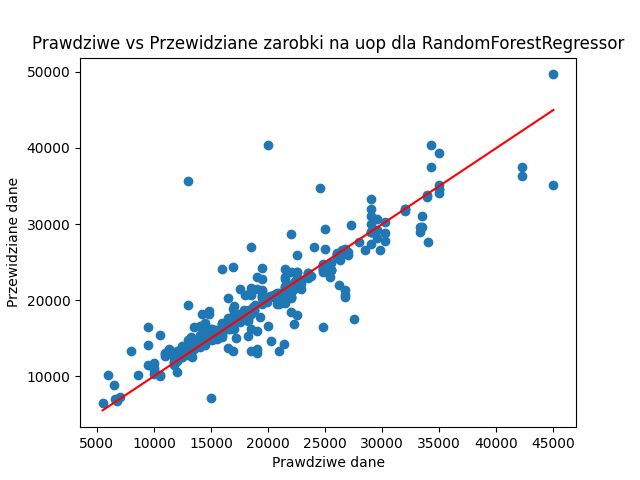
\includegraphics[width=\textwidth]{../analysis/plots/wyniki/0.8&0.2/uop/RandomForestRegressor/scatter.png}
    \caption{Dopasowanie danych przewidzianych do prawdziwych}
\end{figure}

\begin{figure}[H]
    \centering
    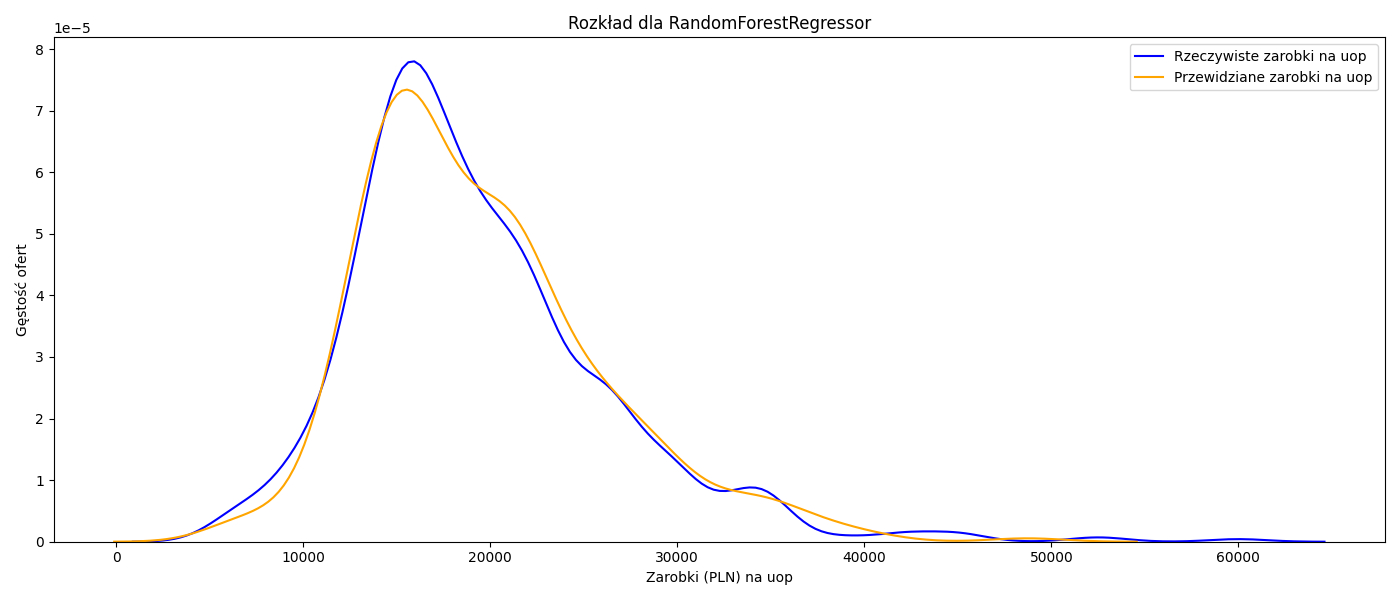
\includegraphics[width=\textwidth]{../analysis/plots/wyniki/0.8&0.2/uop/RandomForestRegressor/salary_dist.png}
    \caption{Rozkład dla przewidzianych i prawdziwych wartości}
\end{figure}

\begin{figure}[H]
    \centering
    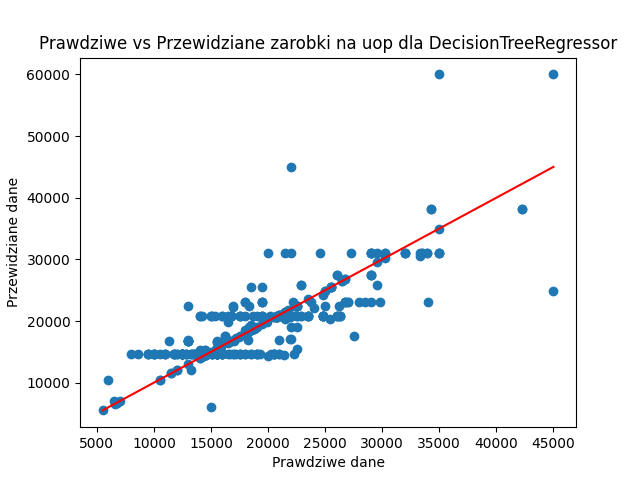
\includegraphics[width=\textwidth]{../analysis/plots/wyniki/0.8&0.2/uop/DecisionTreeRegressor/scatter.png}
    \caption{Dopasowanie danych przewidzianych do prawdziwych}
\end{figure}

\begin{figure}[H]
    \centering
    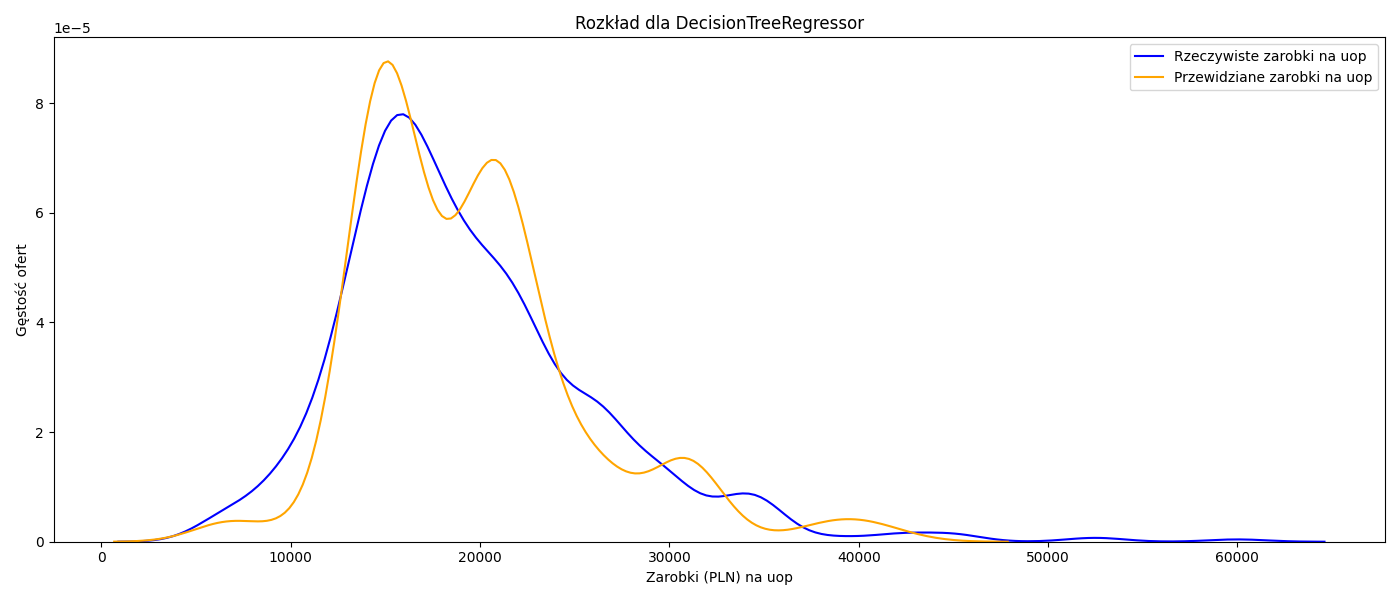
\includegraphics[width=\textwidth]{../analysis/plots/wyniki/0.8&0.2/uop/DecisionTreeRegressor/salary_dist.png}
    \caption{Rozkład dla przewidzianych i prawdziwych wartości}
\end{figure}

\subsubsection{Wyniki dla podziału danych 80:20 dla b2b}

\begin{table}[H]
    \centering
    \begin{tabular}{|c|c|c|c|}
        \hline
        \textbf{Model}        & \textbf{Mean Absolute Error} & \textbf{Root Mean Squared Error} & \textbf{R\textsuperscript{2} Score} \\ \hline
        LinearRegression      & 3636.41                      & 4807.77                          & 0.47                                \\ \hline
        DecisionTreeRegressor & 2624.86                      & 3897.49                          & 0.65                                \\ \hline
        RandomForestRegressor & 1729.25                      & 3104.98                          & 0.78                                \\ \hline
        Ridge                 & 3633.46                      & 4811.16                          & 0.47                                \\ \hline
        Lasso                 & 3634.19                      & 4822.0                           & 0.47                                \\ \hline
    \end{tabular}
\end{table}

\quad W tym przyadku jest tak samo najlepszym okazuje się \texttt{RandomForestRegressor} a następnym
jest \texttt{DecisionTreeRegressor}.


\begin{figure}[H]
    \centering
    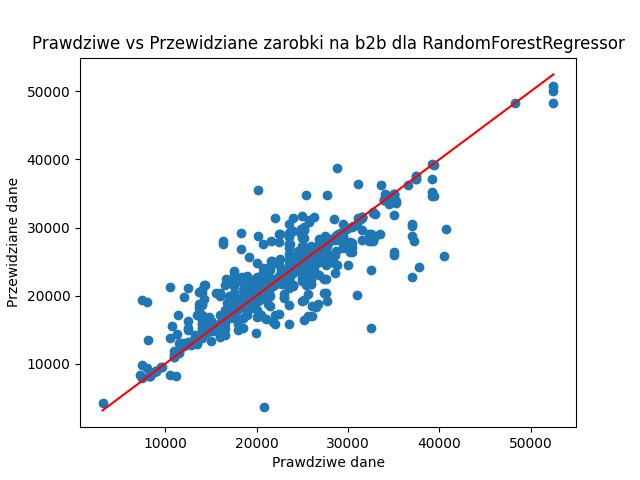
\includegraphics[width=\textwidth]{../analysis/plots/wyniki/0.8&0.2/b2b/RandomForestRegressor/scatter.png}
    \caption{Dopasowanie danych przewidzianych do prawdziwych}
\end{figure}

\begin{figure}[H]
    \centering
    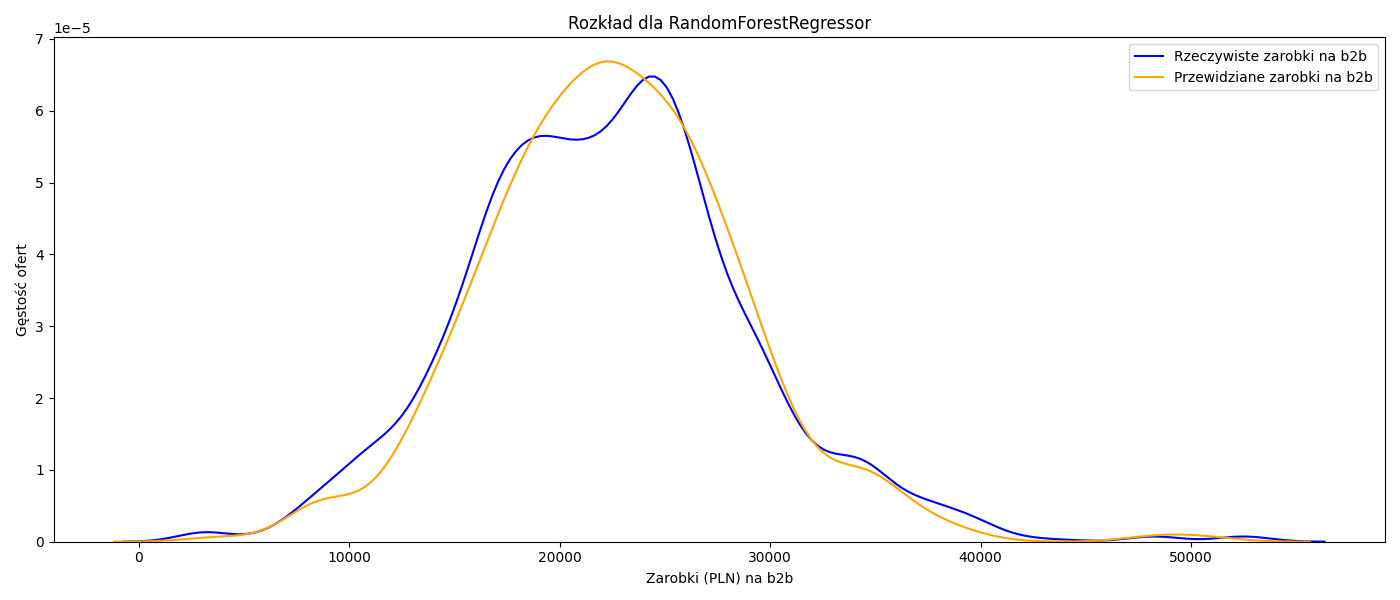
\includegraphics[width=\textwidth]{../analysis/plots/wyniki/0.8&0.2/b2b/RandomForestRegressor/salary_dist.png}
    \caption{Rozkład dla przewidzianych i prawdziwych wartości}
\end{figure}

\begin{figure}[H]
    \centering
    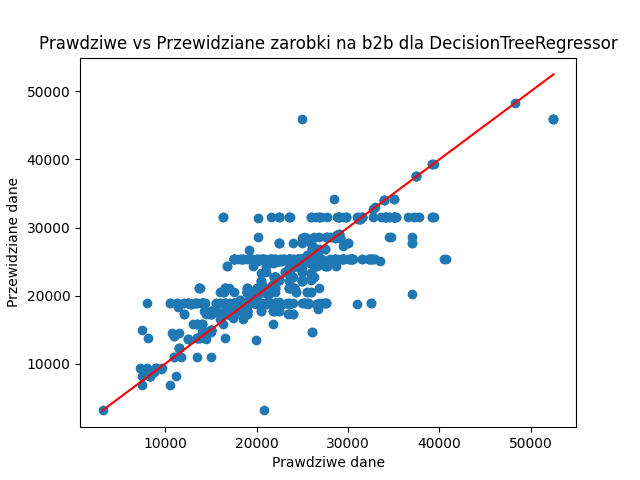
\includegraphics[width=\textwidth]{../analysis/plots/wyniki/0.8&0.2/b2b/DecisionTreeRegressor/scatter.png}
    \caption{Dopasowanie danych przewidzianych do prawdziwych}
\end{figure}

\begin{figure}[H]
    \centering
    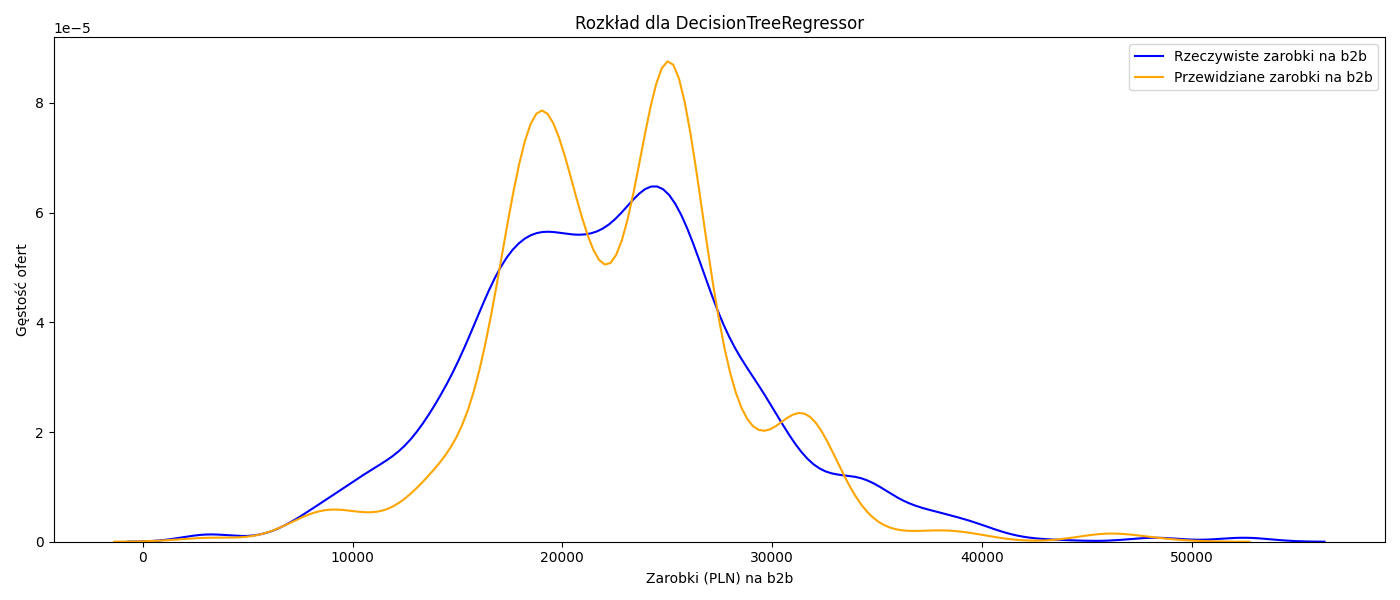
\includegraphics[width=\textwidth]{../analysis/plots/wyniki/0.8&0.2/b2b/DecisionTreeRegressor/salary_dist.png}
    \caption{Rozkład dla przewidzianych i prawdziwych wartości}
\end{figure}


\subsubsection{Podsumowanie wyników dla 80:20}

\quad Wyniki pokazały nam, że najlepszym modelem do przewidywania zarobków od innych danych w ofercie jest \texttt{RandomForestRegressor} z parametrami \texttt{n\_estimators=80},
chociaż błędy były dość wysokie, ale może to wynikać z dużego zakresu pensji oraz mogą być spowodowane małą ilością ofert pracy dla juniorów. Co warto zauważyć,
w najlepszego modelu dane były w miarę skupione w prostej wyznaczającej idealny wynik. Dopasowanie rozkładu było też całkiem dobre, ponieważ
wykresy w większej części nachodziły na siebie. Ostatnia uwaga, model do przewidywania zarobków na umowie jest dokładniejszy niż model przewidujący zarobki na b2b.


\subsubsection{Wyniki dla podziału danych 60:40 dla uop}

\begin{table}[H]
    \centering
    \begin{tabular}{|c|c|c|c|}
        \hline
        \textbf{Model}        & \textbf{Mean Absolute Error} & \textbf{Root Mean Squared Error} & \textbf{R\textsuperscript{2} Score} \\ \hline
        LinearRegression      & 3994.07                      & 5361.73                          & 0.44                                \\ \hline
        DecisionTreeRegressor & 2484.37                      & 3918.8                           & 0.70                                \\ \hline
        RandomForestRegressor & 1762.22                      & 3582.26                          & 0.75                                \\ \hline
        Ridge                 & 3982.56                      & 5360.68                          & 0.44                                \\ \hline
        Lasso                 & 3980.56                      & 5357.41                          & 0.44                                \\ \hline
    \end{tabular}
\end{table}

\begin{figure}[H]
    \centering
    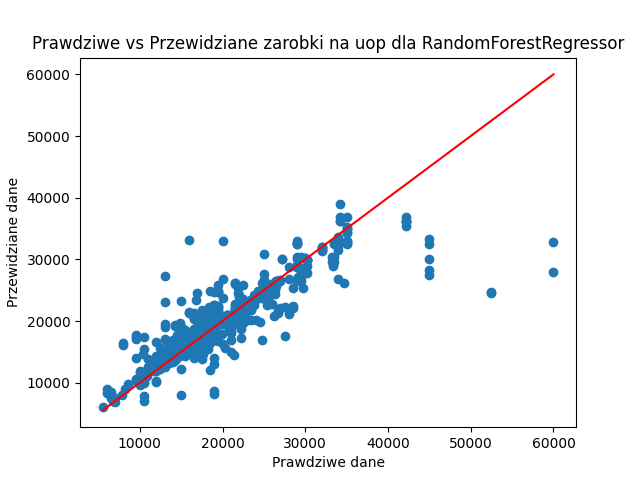
\includegraphics[width=\textwidth]{../analysis/plots/wyniki/0.6&0.4/uop/RandomForestRegressor/scatter.png}
    \caption{Dopasowanie danych przewidzianych do prawdziwych}
\end{figure}

\begin{figure}[H]
    \centering
    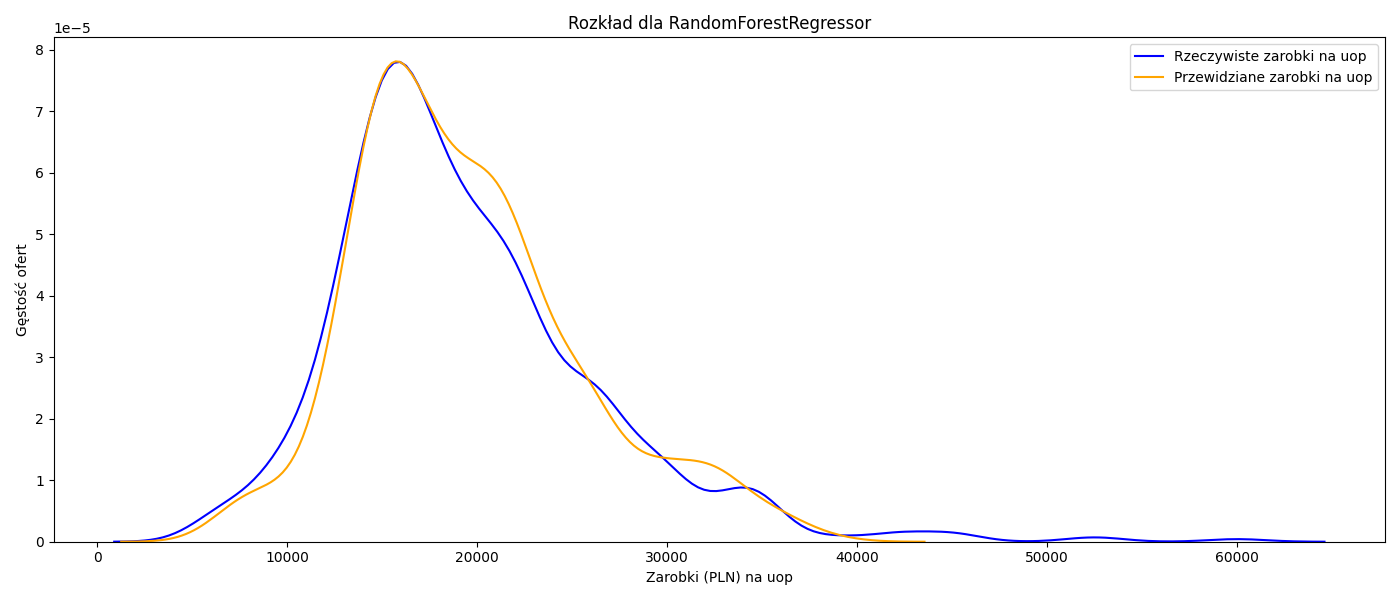
\includegraphics[width=\textwidth]{../analysis/plots/wyniki/0.6&0.4/uop/RandomForestRegressor/salary_dist.png}
    \caption{Rozkład dla przewidzianych i prawdziwych wartości}
\end{figure}

\begin{figure}[H]
    \centering
    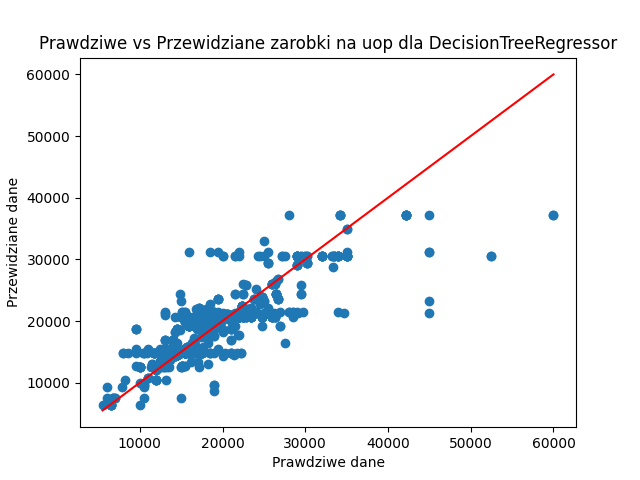
\includegraphics[width=\textwidth]{../analysis/plots/wyniki/0.6&0.4/uop/DecisionTreeRegressor/scatter.png}
    \caption{Dopasowanie danych przewidzianych do prawdziwych}
\end{figure}

\begin{figure}[H]
    \centering
    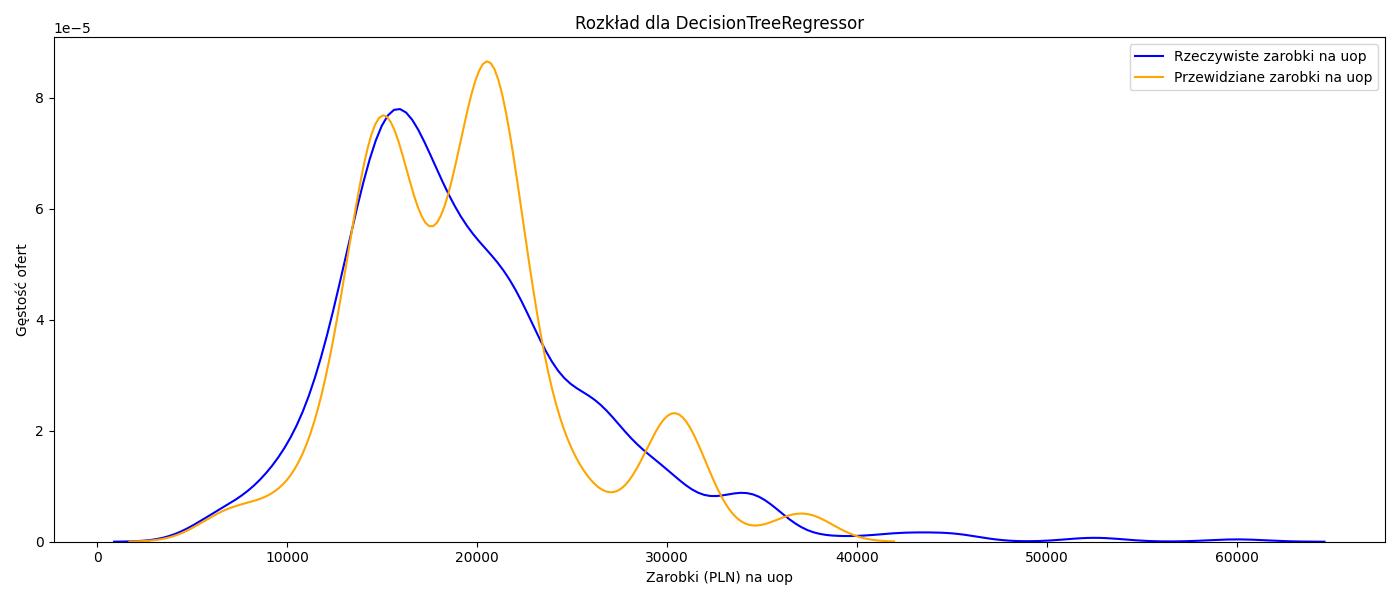
\includegraphics[width=\textwidth]{../analysis/plots/wyniki/0.6&0.4/uop/DecisionTreeRegressor/salary_dist.png}
    \caption{Rozkład dla przewidzianych i prawdziwych wartości}
\end{figure}

\subsubsection{Wyniki dla podziału danych 60:40 dla uop}

\begin{table}[H]
    \centering
    \begin{tabular}{|c|c|c|c|}
        \hline
        \textbf{Model}        & \textbf{Mean Absolute Error} & \textbf{Root Mean Squared Error} & \textbf{R\textsuperscript{2} Score} \\ \hline
        LinearRegression      & 3520.18                      & 4613.03                          & 0.49                                \\ \hline
        DecisionTreeRegressor & 2564.56                      & 3796.84                          & 0.65                                \\ \hline
        RandomForestRegressor & 1896.69                      & 3275.59                          & 0.74                                \\ \hline
        Ridge                 & 3516.78                      & 4611.84                          & 0.49                                \\ \hline
        Lasso                 & 3516.41                      & 4616.76                          & 0.49                                \\ \hline
    \end{tabular}
\end{table}

\begin{figure}[H]
    \centering
    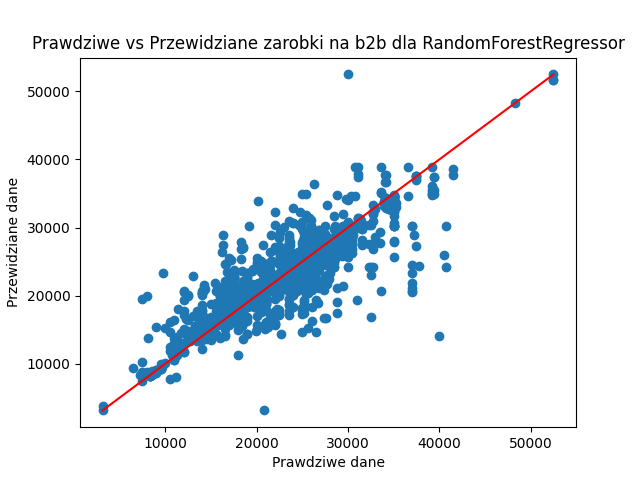
\includegraphics[width=\textwidth]{../analysis/plots/wyniki/0.6&0.4/b2b/RandomForestRegressor/scatter.png}
    \caption{Dopasowanie danych przewidzianych do prawdziwych}
\end{figure}

\begin{figure}[H]
    \centering
    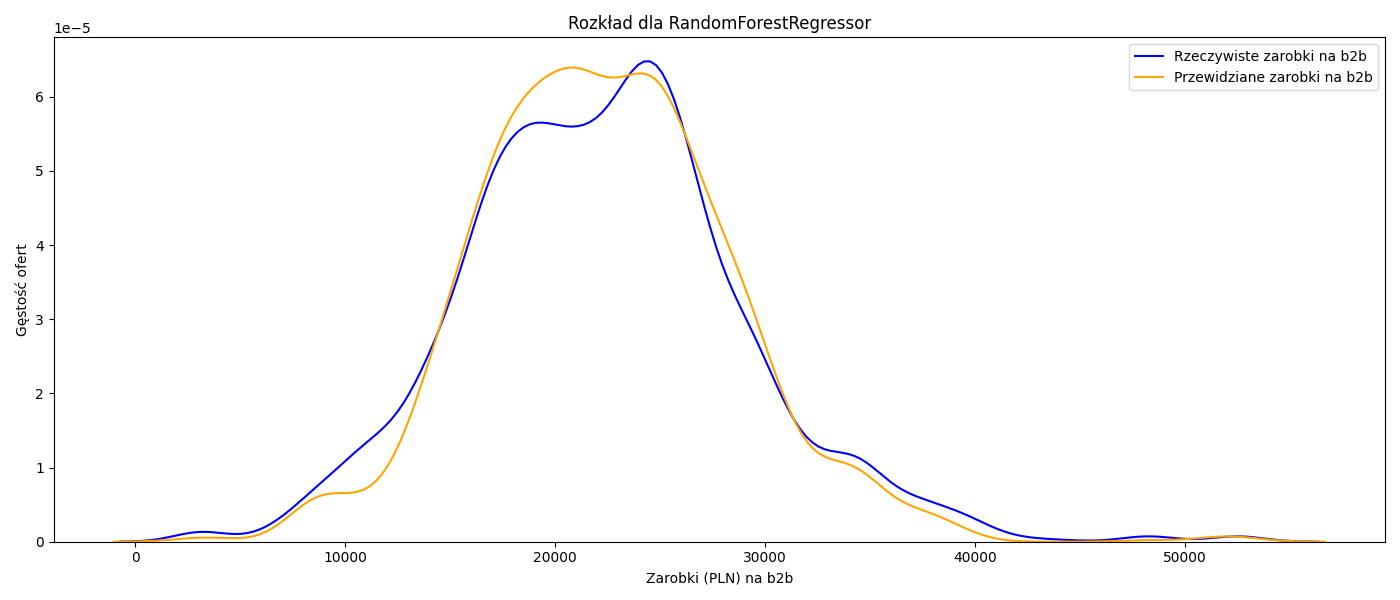
\includegraphics[width=\textwidth]{../analysis/plots/wyniki/0.6&0.4/b2b/RandomForestRegressor/salary_dist.png}
    \caption{Rozkład dla przewidzianych i prawdziwych wartości}
\end{figure}

\begin{figure}[H]
    \centering
    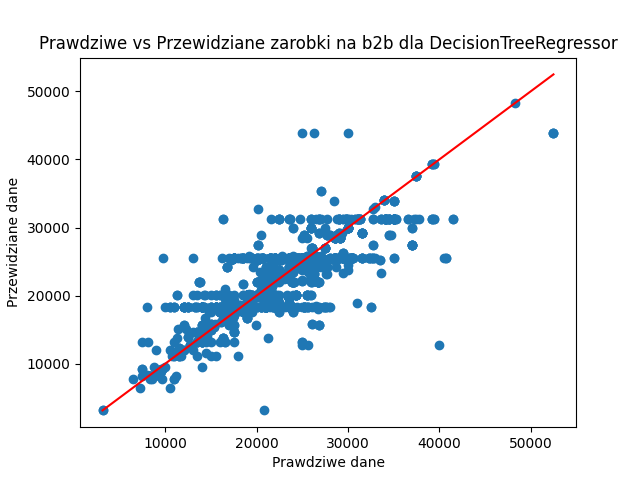
\includegraphics[width=\textwidth]{../analysis/plots/wyniki/0.6&0.4/b2b/DecisionTreeRegressor/scatter.png}
    \caption{Dopasowanie danych przewidzianych do prawdziwych}
\end{figure}

\begin{figure}[H]
    \centering
    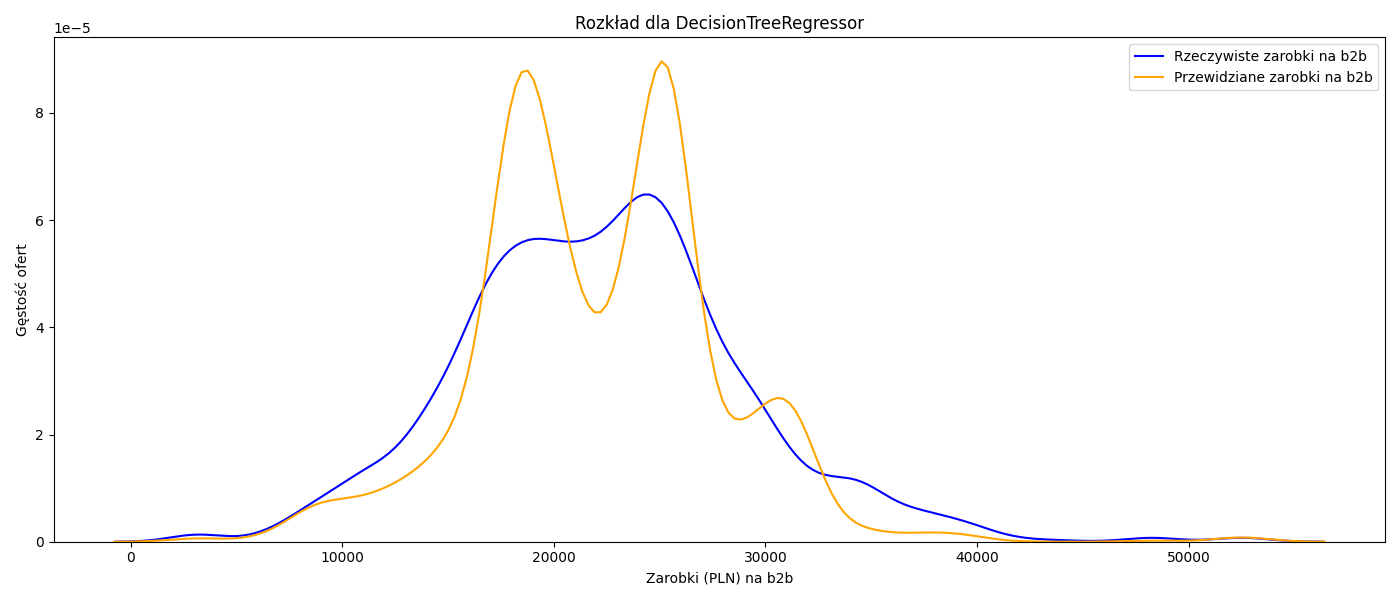
\includegraphics[width=\textwidth]{../analysis/plots/wyniki/0.6&0.4/b2b/DecisionTreeRegressor/salary_dist.png}
    \caption{Rozkład dla przewidzianych i prawdziwych wartości}
\end{figure}


\subsubsection{Podsumowanie wyników dla 60:40}


\quad Wyniki dla tej podziałki są na pewno mniej precyzyjne jeśli chodzi o \textbf{RMSE}, ale dla takiego podzielenia daynch znów najlepszymi modelami okazały się modele
kolejno \texttt{RandomForestRegressor} oraz \texttt{DecisionTreeRegressor}.

\section{Podsumowanie}
\quad Podsumowując, jeśli chodzi o stworzenie modelu to najlepszym będzie \newline \texttt{RandomForestRegressor(n\_estimators=80)},
ponieważ dawał najmniejsze błędy chociaż i tak w skali zarobków nie były one małe.
Do uczenia okazało się, że lepiej wybrać podziałkę 80:20, 80\% dane treningowe a 20\% dane testowe. Wydaje mi się również, że aby uzyskać lepsze wyniki,
należałoby zaktualizować zbiór danych o nowe oferty (głównie oferty dla juniorów).
Oczywiście model model może być jeszcze lepiej rozwinięty jeśli dodane zostałby nowe cechy np. stopień naukowy lub nowe 
technologie lub większe wyspecyfikowanie technologii.

\quad Podczas pracy również można było sporządzić wykres, który przedstawiał najważniejsze zmienne w sensie wypływu na wynagrodzenie.

\begin{figure}[H]
    \centering
    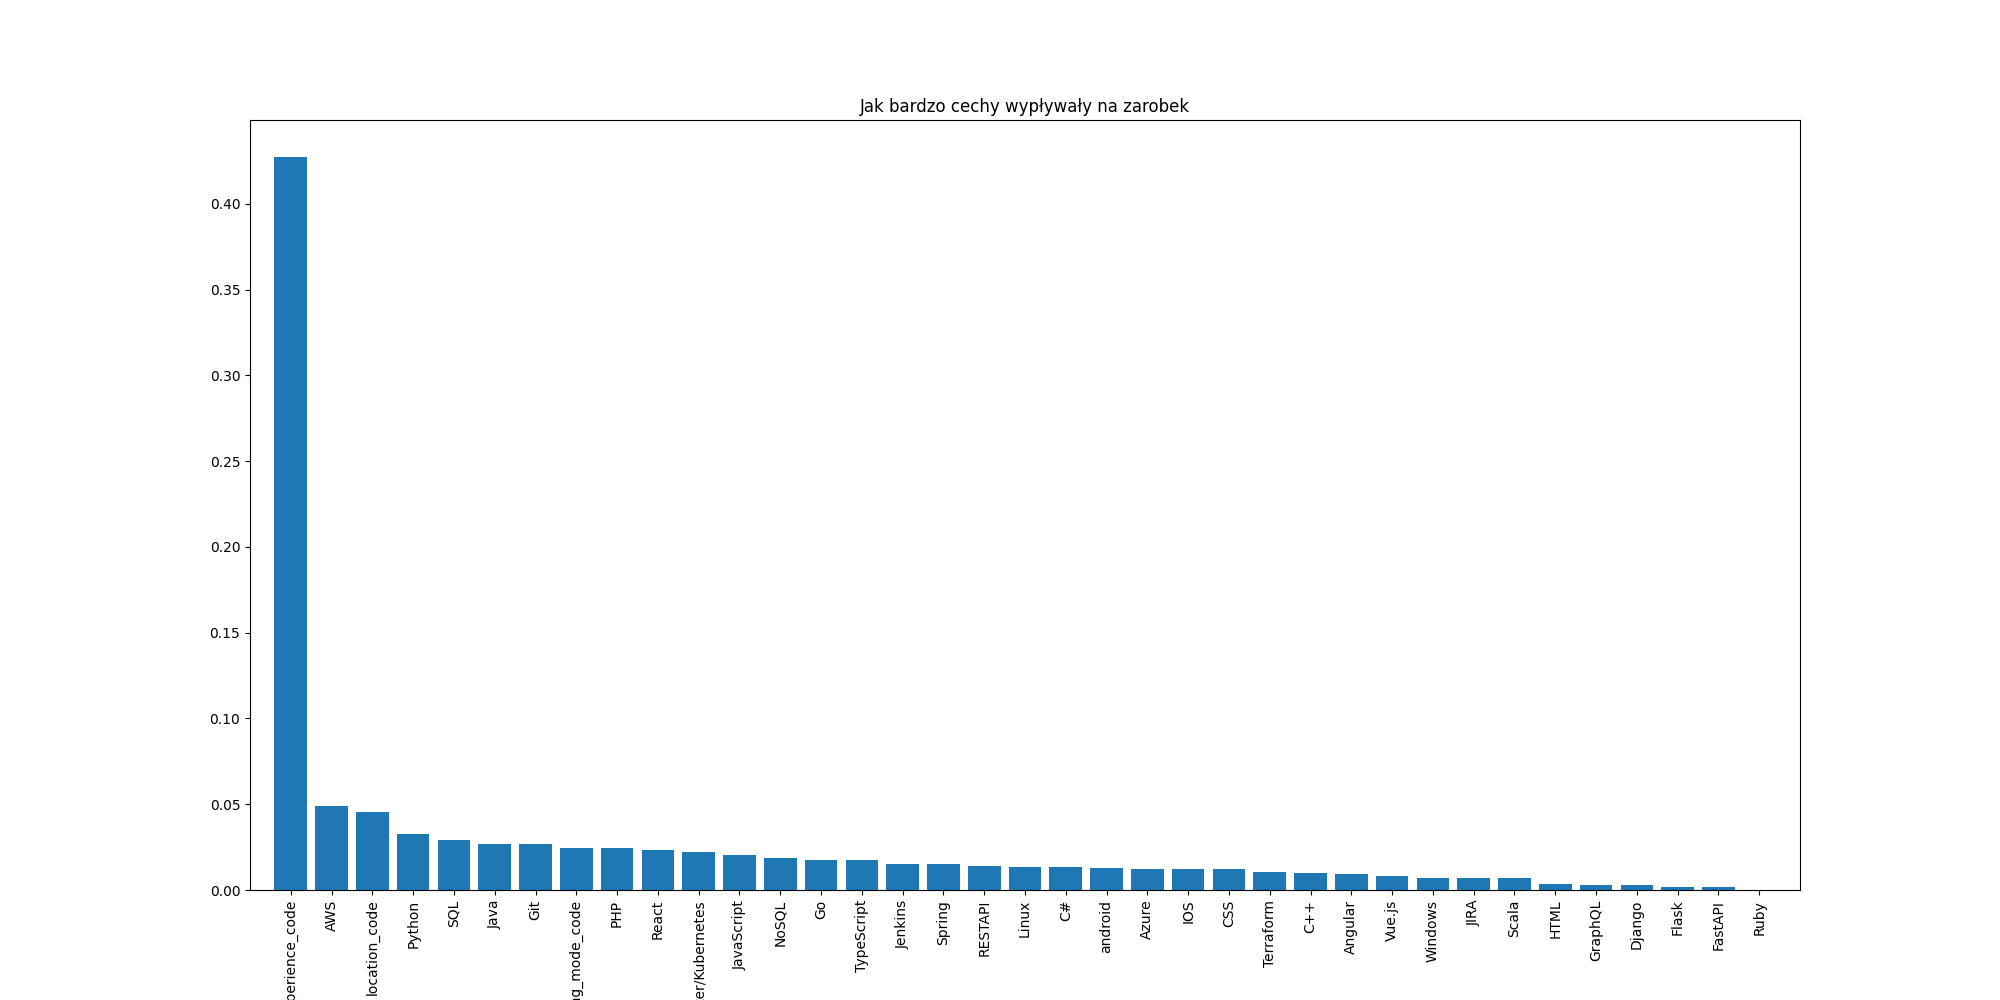
\includegraphics[width=\textwidth]{../analysis/plots/wyniki/importance_of_vars.png}
    \caption{Zmienne mające wypłw na wynagrodzenie w ofercie pracy}
\end{figure}

\quad Jak łatwo zauważyć, doświadczenie miało największy wpływ na przewidywaną wartość.
Kolejnymi zmiennymi, które mogły zaskoczyć był np. \textbf{AWS, SQL, Python}. 

\section{Testowanie wyuczonego modelu}

\quad Tak jak już wcześniej wspomniałem model, który uznałem za odpowiedni, czyli popełniający najmniejszy błąd
spośród wszystkich to \texttt{RandoForestRegressor(n_estimators=80)}, dla podziałki 80:20. 
Przetestuję model, który przewidzi mi pensje na b2b i na umowie o pracę w zależności od
moich technologii, które znam. Zakładam, że test może dać trochę słabe wyniki, ponieważ
model będzie musiał przewidzieć zarobki dla takich danych: 




\end{document}


